\header[v]{
    \section{Le chant des étudiants Wallons} \label{le-chant-des-etudiants-wallons}
    %
    
    \insertComment{Sur l'air du "Grenadier des Flandres".}{Datant d'avant 1938, ce chant met en valeur Gambrinus (Jan primus), roi mythique de Flandre et Brabant, aujourd'hui symbole des amateurs de bière.\\
    Paru dans le journal L'Étudiant Libéral liégeois de 1938 (n°10, p. 2, col. 5), on y lit : "Ce chant, qui jouit actuellement d'une très grande vogue, est dû à la plume d'Antoine Clexe, étudiant montois qui coula autrefois quelques bonnes années à Liége. La musique est de notre compatriote Hillier, ancien étudiant, actuellement chef d'orchestre à Vichy."}
    %
    %
}

\enluminure{4}{\href{https://www.youtube.com/watch?v=WnDt6agxyBY}{Q}}{ue} jusque tout au bord
\\L'on remplisse nos verres;
\\Qu'on les remplisse encore
\\De la même manière,
\\Car nous sommes les plus forts
\\Buveurs de blonde bière.
\\\\\textbf{Refrain :}
\\Car nous restons, de gais Wallons !
\\Dignes de nos aïeux, Nom de Dieu
\\Car nous sommes comme eux, Nom de Dieu
\\Disciples de Bacchus et du roi Gambrinus !
\\\\Nous ne craignons pas ceux
\\Qui dans la nuit nous guettent :
\\Les Flamands et les gueux
\\A la taille d'athlètes,
\\Ni même que les cieux
\\Nous tombent sur la tête.
\\\\Nous assistons aux cours
\\Parfois avec courage.
\\Nous bloquons certains jours
\\Sans trop de surmenage,
\\Mais nous buvons toujours
\\Avec la même rage.
\\\\Quand nous fermerons l'oeil,
\\Au soir de la bataille,
\\Pour fêter notre deuil
\\Qu'on fasse une guindaille.
\\Et pour notre cercueil
\\Qu'on prenne une futaille.
\\\\Et quand nous paraîtrons
\\Devant le grand Saint Pierre,
\\Sans crainte nous lui dirons:
\\"Autrefois sur la terre,
\\Grand saint, nous n'aimions
\\Que les femmes et la bière !".
\\\\Et quand nous serons pleins
\\Nous irons jusqu'en Flandre
\\Armés de nos gourdins
\\Pour faire un bel esclandre
\\Et montrer aux Flamandes
\\Comment c'qu'on sait les prendre !
\\\\Puisque ces calottins 
\\Nous abreuvent d'injures
\\Qu'on leur dise en latin
\\L'horreur de leur parjure
\\Des moines, des sacristains
\\Et des Saintes Ecritures ! 
\\\\\textbf{Refrain} \{ ter
\begin{center}
   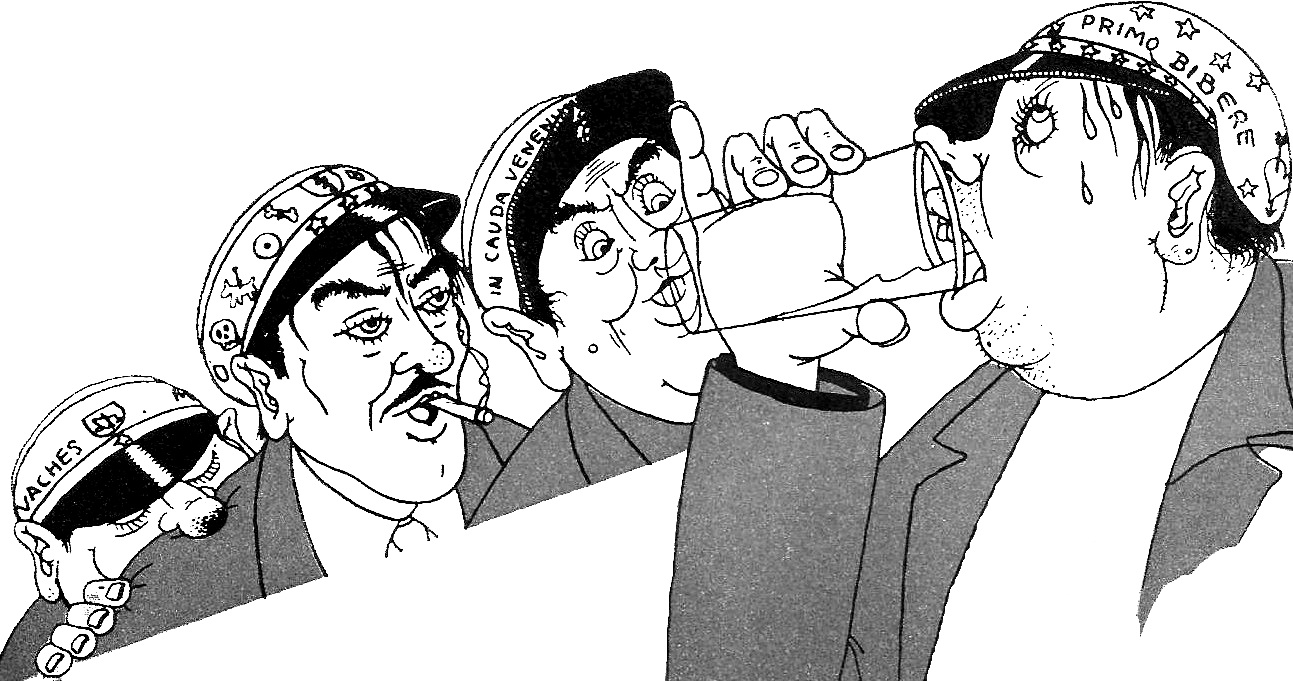
\includegraphics[width=0.8\textwidth]{images/Wallon.jpg}
 \end{center}
\breakpage